\section{Problem description and analysis}
\label{sec:Problem}
In this section, we first present the system model, then the problem formulation, and finally analyze the problem complexity. 
\subsection{System model}
A shared risk link group (SRLG) is a group of links that share a component whose failure causes the failure of all links in the group. %Depending on the network types, the shared physical resource may refer to the conduit of an optical network, the cable of smart grids and Internet, the underlying physical structure of an overlay network. Our divide and conquer algorithm is general and applicable for any network types.

An example of such a component is the fiber conduit \cite{bhandari1994optimal} in optical networks, where several optical links may be placed side-by-side in one single conduit, as illustrated in Fig.\ref{fig:SRLGgraph}. Links (1,2), (3,2) and (3,4) are placed inside a single conduit, while links (3,2) and (3,4) also share another single conduit. If a conduit gets cut, the corresponding links will fail. Each conduit corresponds a SRLG.  Other example applications of SRLGs are the correlated congestion of transportation networks and cascading failures of power grid networks \cite{coudert2007shared}. A link can belong to multiple SRLGs.
\begin{figure}[htbp]
\centering
\subfigure[Physical topology with conduit]{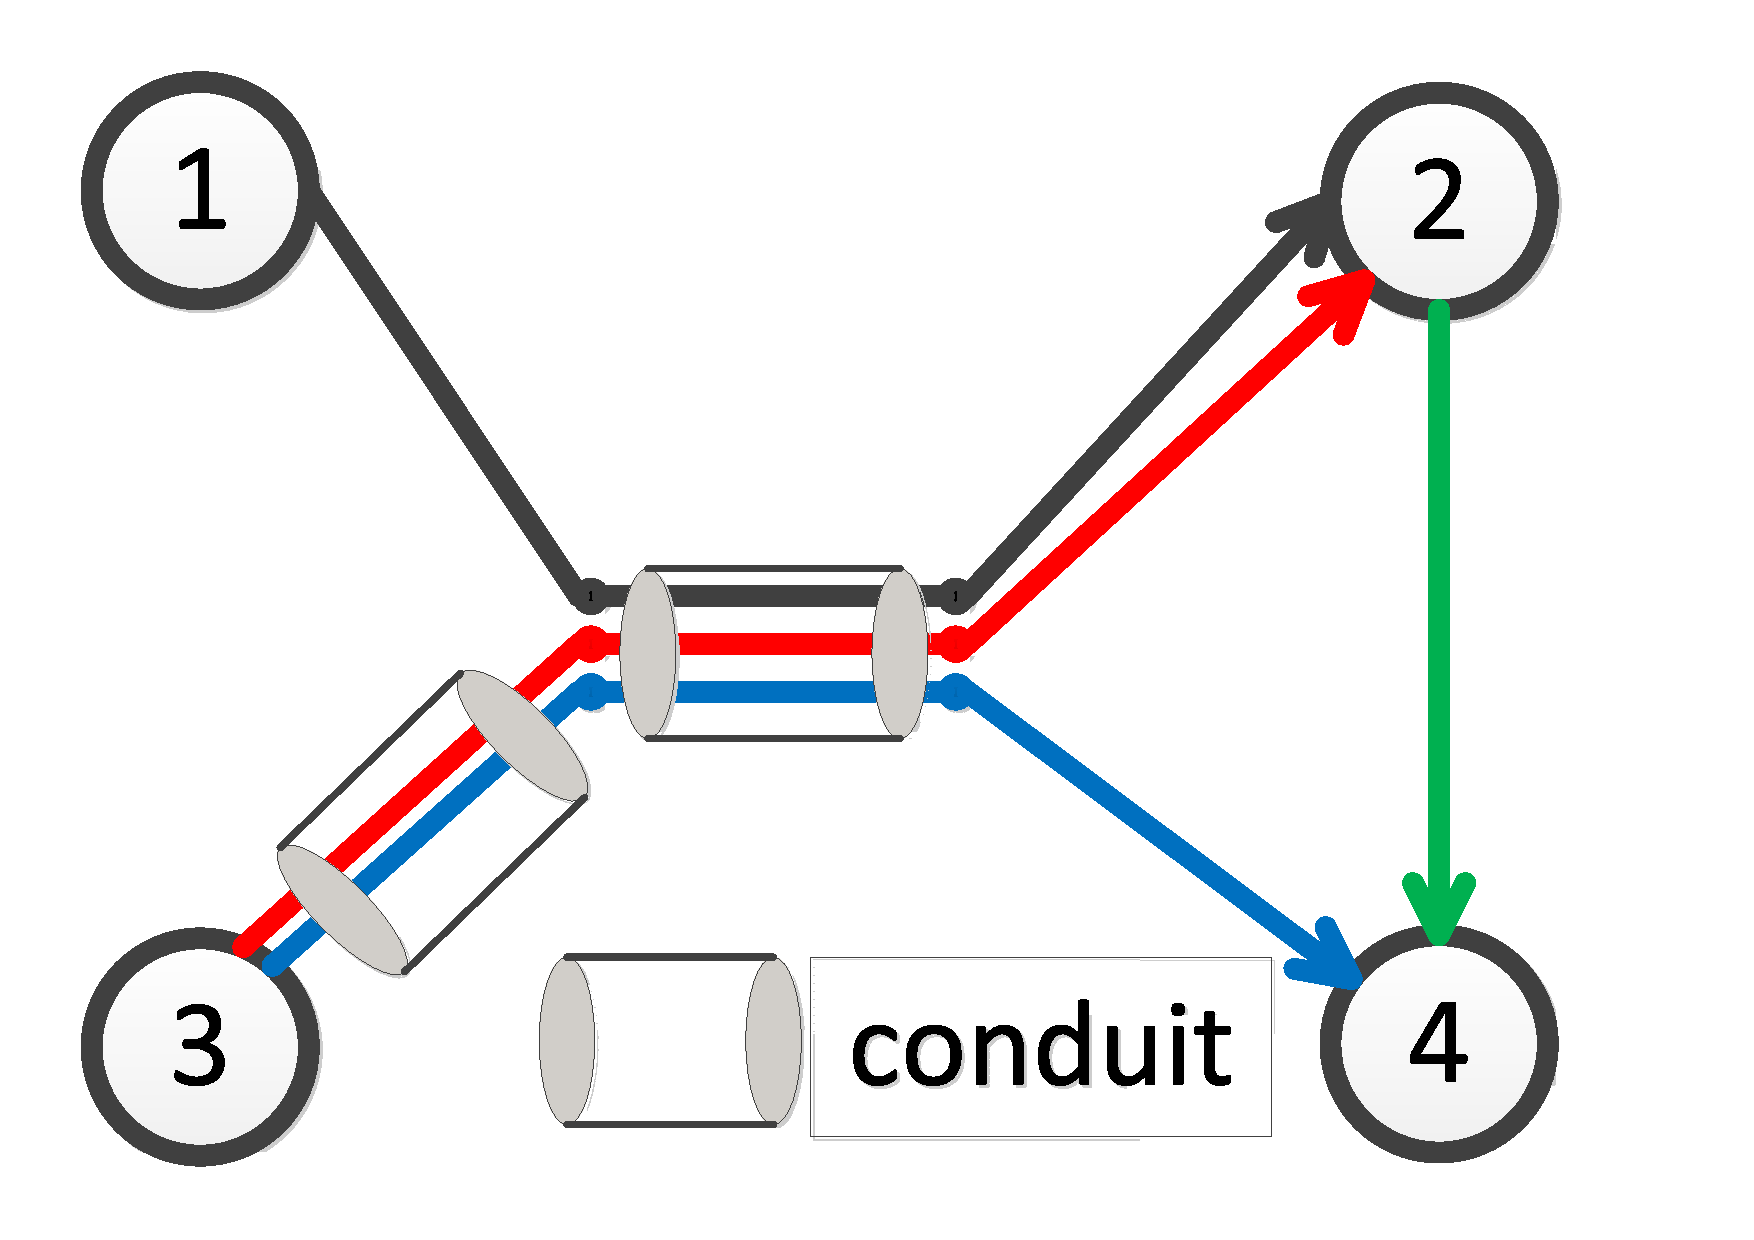
\includegraphics[width=1.25 in]{franz/PhysicalGraph}
}
\subfigure[Network Graph]{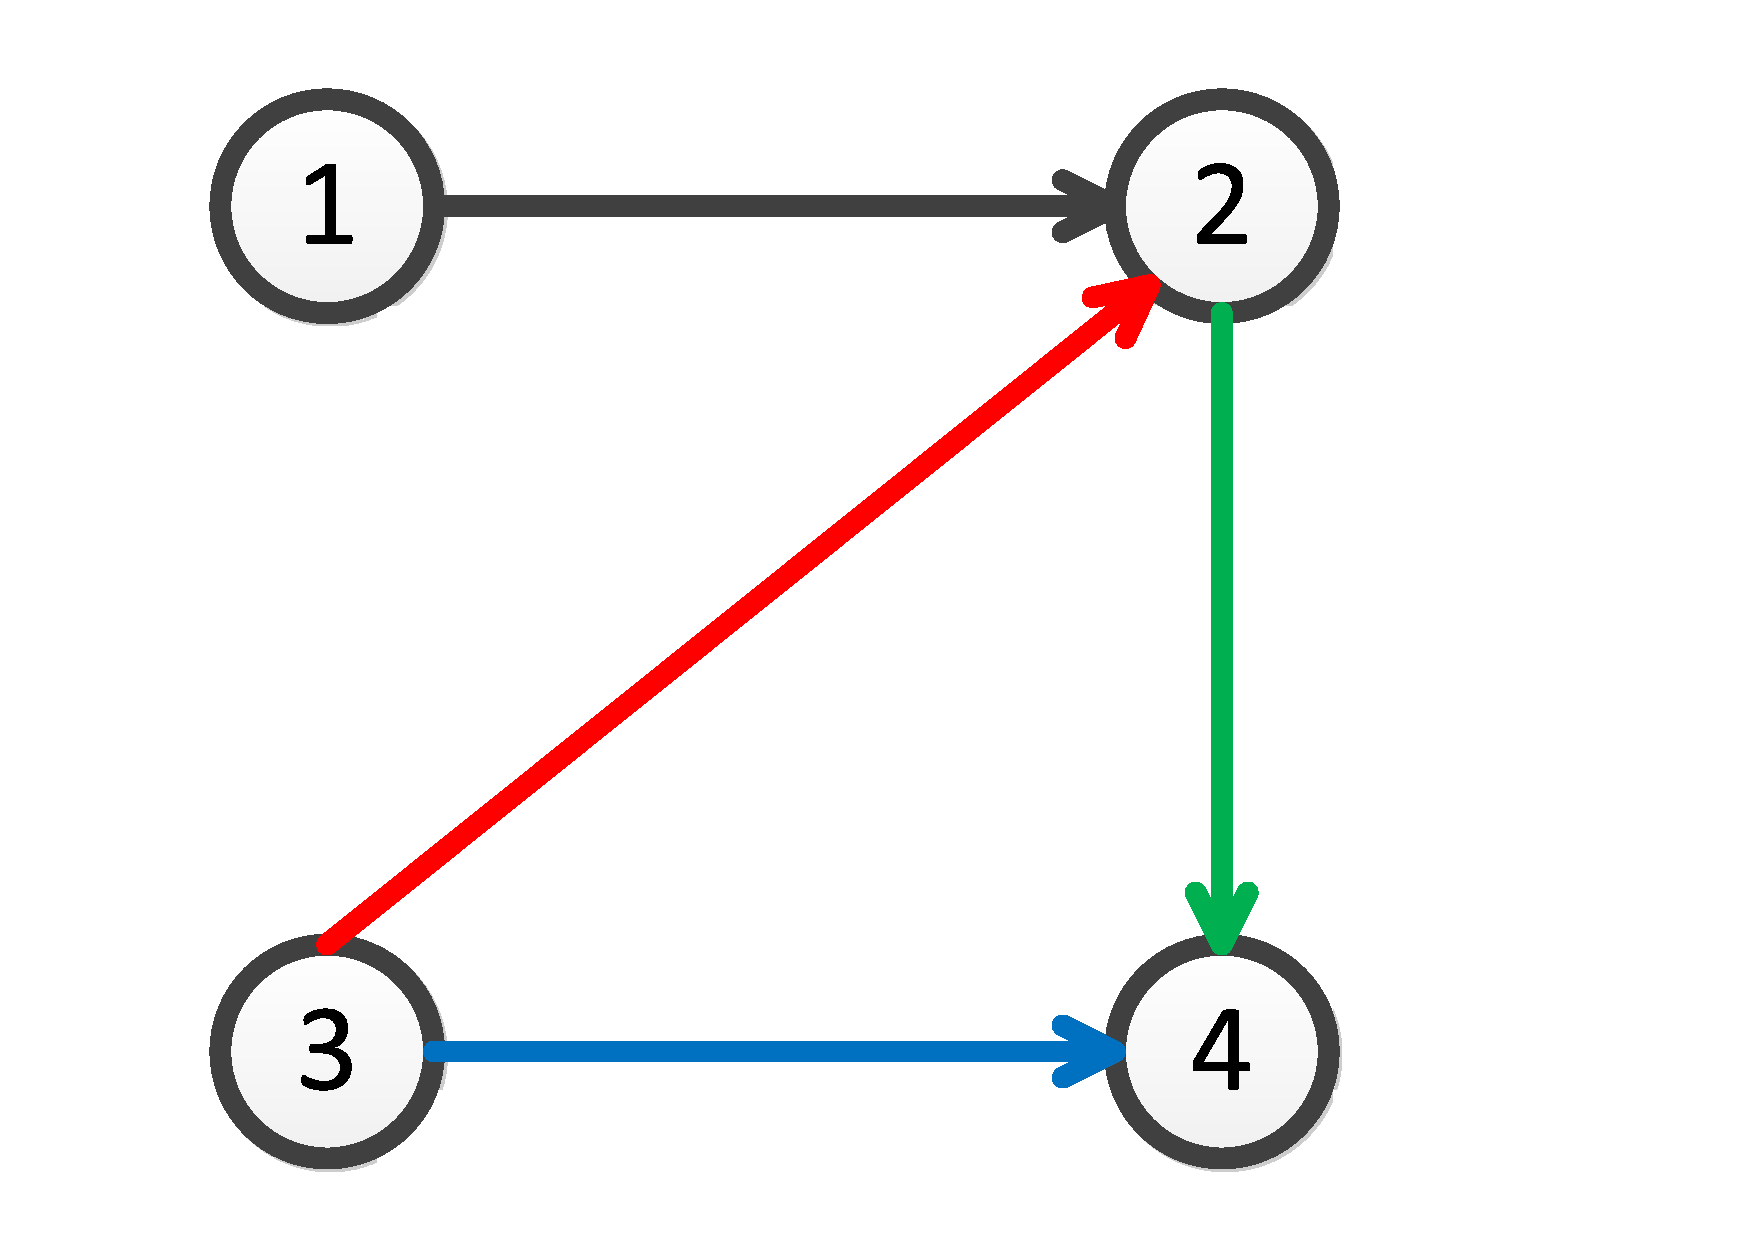
\includegraphics[width=0.9 in]{franz/VirtualGraph}
}
\caption{Example of shared risk link group(SRLG)}\label{fig:SRLGgraph}
\label{fig:Logic shift operation}
\end{figure}

Let $\mathbb{R}$ be the risk (failure) set in the network. Each risk may correspond to a conduit cut, a fiber cut, a card failure at a node, a software failure, or any combination of these factors. For $r_i \in \mathbb{R}$, its SRLG is the link set associated with risk $r_i$, denoted as $\mathbb{R}_{r_i}$, where $1\leq i\leq \chi$ and $\chi=|{\mathbb{R}}|$ is the number of risks/SRLGs.  In Fig.\ref{fig:CompositeGraph}(a), the network includes five SRLGs $\mathbb{R}_{r_1}=\{e_1,e_9\}$, $\mathbb{R}_{r_2}=\{e_2,e_3,e_{19}\}$, $\mathbb{R}_{r_3}=\{e_2,e_4,e_{11},e_{17}\}$, $\mathbb{R}_{r_4}=\{e_5,e_{13}\}$, $\mathbb{R}_{r_5}=\{e_{15},e_{18}\}$. In this example, link $e_2$ is in two SRLGs $\mathbb{R}_{r_2}$ and $\mathbb{R}_{r_3}$.

A network is often represented as a graph $G(\mathbb{V},\mathbb{E})$, where $\mathbb{V}$ is the set of $|\mathbb{V}|$ nodes (which for instance represent routers) and $\mathbb{E}$ is the set of $|\mathbb{E}|$ links (which for instance represent optical fiber lines or radio channels). Links may be characterized by weights representing for instance their delay, length, or cost. For a link $e_i$, we denote the weight of the link as $w_{e_i}$. The weight of a path $P$ is denoted as $w_P=\sum\limits_{e_i\in \mathbb{P}}w_{e_i}$, which is the sum of  the weight of each link in the path.

Let $r_P$ denote the risk set that impacts a path $P$, that is $r_P=\{r\in \mathbb{R}$: path $P$ contains links in $\mathbb{R}_r\}$. In Fig.\ref{fig:CompositeGraph}(c), the link set on the AP is $\mathbb{AP}=\{e_1,e_2,e_3,e_4,e_5,e_6,e_7,e_8\}$ with $e_1\in \mathbb{R}_{r_1}$, $e_2\in \mathbb{R}_{r_2}$, $e_2\in \mathbb{R}_{r_3}$, $e_3\in \mathbb{R}_{r_2}$, $e_4\in \mathbb{R}_{r_3}$, $e_5\in \mathbb{R}_{r_4}$,  the risk set of AP is ${r}_{{AP}}=\{r_1, r_2, r_3, r_4\}$. $\mathbb{\mathbb{ER}}$ denotes the set of links not belonging to AP that share the common risks with AP. In Fig.\ref{fig:CompositeGraph}(c), $\mathbb{\mathbb{ER}}=\{e_9,e_{11},e_{17},e_{13},e_{19}\}$.

SRLG-disjoint paths share no common risks among themselves, that is, the failure of a path due to a risk would not affect other paths. Fig.\ref{fig:CompositeGraph}(b) shows two SRLG-disjoint paths, denoted as AP and BP. As these two paths share no common risk, if AP fails, BP can still work.
\subsection{Problem formulation}
Given a source node $s$ and a destination node $d$, this paper focuses on finding  two SRLG-disjoint paths from $s$ to $d$ for path protection. Before we present the problem formulation, we first introduce some necessary notation.
%
%$x_{e_i}^{AP}=\{0,1\}$ and $x_{e_i}^{BP}=\{0,1\}$ are the binary variables to specify whether or not the link $e_i$ in active in AP and BP, respectively.
%
%
%
%$x_{e_i}^{AP}=\{0,1\}$ denote whether link $e_i$ belong to path AP, $x_{e_i}^{BP}=\{0,1\}$ denote whether link $e_i$ belong to path BP



$u=[u_v]^T_{v\in \mathbb{V}}$ is the vector \rev{that identifies node types, where}
%source destination column vector, where
${{u_v}} = \left\{ {\begin{array}{*{20}{c}}
1&{if\ v=s}\\
{ - 1}&{if\ v=d}\\
0&{otherwise}
\end{array}} \right.$


$A=[a_{v,e_i}]_{|\mathbb{V}|\times |\mathbb{E}|}$ is \rev{a matrix to identify the node edge relationship,} 
%is the node edge incidence matrix, 
where ${a_{v,e_i}} = \left\{ {\begin{array}{*{20}{c}}
1&{if\ link\ e_i\ originates\ from\ node\ v}\\
{ - 1}&{if\ link\ e_i\ terminates\ at\ node\ v}\\
0&{otherwise}
\end{array}} \right.$

%$H=[h_{r,e}]_{R\times E}$ the risk-edge incidence matrix, where ${\rm{h_{r,e}}} = \left\{ {\begin{array}{*{20}{c}}
%1&{if\ edge\ e \in \mathbb{R}_r}\\
%0&{otherwise}
%\end{array}} \right.$

$x^{AP} = [x_{e_i}^{AP}]^T_{e_i\in \mathbb{E}}$ is the column vector  where ${x_{e_i}^{AP}}$ is the binary variable  to specify whether or not link ${e_i}$ \rev{is on the} path AP, that is,  ${x_{e_i}^{AP}} = \left\{ {\begin{array}{*{20}{c}}
1&{if\ link\ e_i \in \mathbb{AP}}\\
0&{otherwise}
\end{array}} \right.$
%$x_{e_i}^{AP}=\{0,1\}$ denote whether link $e_i$ belong to path AP,

$x^{BP}=[x_{e_i}^{BP}]^T_{e_i\in \mathbb{E}}$ is the column vector where ${x_{e_i}^{BP}}$ is the binary variable  to specify whether or not  link ${e_i}$ is \rev{on the} path BP, that is, ${x_{e_i}^{BP}} = \left\{ {\begin{array}{*{20}{c}}
1&{if\ link\ e_i \in \mathbb{BP}}\\
0&{otherwise}
\end{array}} \right.$
%$x_{e_i}^{BP}=\{0,1\}$ denote whether link $e_i$ belong to path BP


\revtao{Using above notations,} the path weight of AP and BP can be expressed as
$w_{AP}=\sum\limits_{e_i\in \mathbb{E}}w_{e_i}x_{e_i}^{AP}$ and $w_{BP}=\sum\limits_{e_i\in \mathbb{E}}w_{e_i}x_{e_i}^{BP}$, respectively. The  risk set of AP and BP can be expressed as $r_{AP}=\{r|{x_{e_i}^{AP}}=1, e_i \in \mathbb{R}_r\}$ and
$r_{BP}=\{r|{x_{e_i}^{BP}}=1, e_i \in \mathbb{R}_r\}$, respectively. 

\textbf{Min-Min SRLG-disjoint routing problem.} Given a graph $G(\mathbb{V},\mathbb{E})$, a weight $w_{e_i}$ associated with each link $e_i\in \mathbb{E}$, a source  $s$ and a destination  $d$,  find a pair of SRLG disjoint paths from $s$ to $d$ (denoted as $AP$ and $BP$), \del{thus} that  the smallest path \rev{weights of both} disjoint paths is minimized, that is,

\begin{equation}
\begin{array}{*{20}{c}}
    \min\limits_{x^{AP}_{e_i}, x^{BP}_{e_i}} & { \left( {w_{AP},w_{BP}} \right)}\\
   {subject\ to} & A\times x^{AP}=u  \\
   {} & A\times x^{BP}=u \\
   {} & 0 \leq x^{AP}_{e_i}+x^{BP}_{e_i}\leq 1\\
   {} & {r_{AP}} \cap {r_{BP}}{\rm{ = }}\phi \\
   {} & x^{AP}_{e_i}, x^{BP}_{e_i} \in {\rm{\{ 0,1\} }}
\end{array}
\label{eq:problem definition}
\end{equation}

In Eq.(\ref{eq:problem definition}),  $A\times x^{AP}=u$ and $A\times x^{BP}=u$ are the  routing constraints  guaranteeing the flow conservation from node $s$ to $d$ along the path. As path AP and BP share the same source node and destination node, \del{therefore,} $A\times x^{AP}=A\times x^{BP}=u$. \rev{The constraint} $0 \leq x^{AP}_{e_i}+x^{BP}_{e_i}\leq 1$  is utilized to guarantee that any link $e_i$ can be active at most in one of the path pair. ${r_{AP}} \cap {r_{BP}}{\rm{ = }}\phi$ is \rev{applied} to guarantee that the path pair AP and BP are SRLG-disjoint\del{ paths}. $x^{AP}_{e_i}$ and $x^{BP}_{e_i}$ are the  binary  decision  variables. Obviously, \rev{the} problem in Eq.(\ref{eq:problem definition}) is an  ILP (integer linear programming) problem.

%$w_{e_i}$ denote the cost of edge $e_i\in \mathbb{E}$, $x_{e_i}^{AP}=\{0,1\}$ denote whether link $e_i$ belong to path AP, $x_{e_i}^{BP}=\{0,1\}$ denote whether link $e_i$ belong to path BP, $u(e_i)$ denote composed nodes of link $e_i$. $w_{AP}=\sum\limits_{e_i\in \mathbb{E}}w_{e_i}*x_{e_i}^{AP}$ denote path weights of AP.  $w_{BP}=\sum\limits_{e_i\in \mathbb{E}}w_{e_i}*x_{e_i}^{BP}$ denote path weights of BP. $r_{AP}=\{r|{e_i}\in \mathbb{AP},e_i \in \mathbb{R}_r\}$, $r_{BP}=\{r|{e_i}\in \mathbb{BP},e_i \in \mathbb{R}_r\}$. $f_{u,v}^{AP}={0,1}$ denote where exist a link $e_i \in \mathbb{AP}$ originate from node $u$ to terminal node $v$. $f_{u,v}^{BP}={0,1}$ denote where exist a link $e_i \in \mathbb{BP}$ originate from node $u$ to terminal node $v$.
%
%\begin{equation*}
%\begin{array}{*{20}{c}}
%    \min & { \left( {w_{AP},w_{BP}} \right)}\\
%   {subject\ to} & \sum\limits_{v\in \mathbb{V}}f_{u(e_i),v}^{AP}-\sum\limits_{v\in \mathbb{V}}f_{v,u(e_i)}^{AP}=1(if\ u(e_i)=s)& (1) \\
%   {} & \sum\limits_{v\in \mathbb{V}}f_{u(e_i),v}^{AP}-\sum\limits_{v\in \mathbb{V}}f_{v,u(e_i)}^{AP}=-1(if\ u(e_i)=d)& (1) \\
%   {} & \sum\limits_{v\in \mathbb{V}}f_{u(e_i),v}^{AP}-\sum\limits_{v\in \mathbb{V}}f_{v,u(e_i)}^{AP}=0(if\ u(e_i)\neq s\ and\ u(e_i)\neq d)& (1) \\
%   {} & \sum\limits_{v\in \mathbb{V}}f_{u(e_i),v}^{BP}-\sum\limits_{v\in \mathbb{V}}f_{v,u(e_i)}^{BP}=1(if\ u(e_i)=s)& (1) \\
%   {} & \sum\limits_{v\in \mathbb{V}}f_{u(e_i),v}^{BP}-\sum\limits_{v\in \mathbb{V}}f_{v,u(e_i)}^{BP}=-1(if\ u(e_i)=d)& (1) \\
%   {} & \sum\limits_{v\in \mathbb{V}}f_{u(e_i),v}^{BP}-\sum\limits_{v\in \mathbb{V}}f_{v,u(e_i)}^{BP}=0(if\ u(e_i)\neq s\ and\ u(e_i)\neq d)& (1) \\
%   {} & 0 \leq x^{AP}_{e_i}+x^{BP}_{e_i}\leq 1(x^{AP}_{e_i}=\{0,1\},x^{BP}_{e_i}=\{0,1\})& (2)\\
%   {} & {r_{AP}} \cap {r_{BP}}{\rm{ = }}\phi& (3) \\
%\end{array}
%\label{eq:problem definition}
%\end{equation*}
%
%
%
%%\revtao{review's advice: It was also mentioned that "For multiple SRLG-disjoint paths, the failure of a path due to a risk would not affect other paths", it would be nice to give an example using Fig. 3.}
%
%\textbf{Min-Min SRLG-disjoint routing problem.} Given a graph $G(\mathbb{V},\mathbb{E})$, a weight $w_{e_i}$ associated with each link $e_i\in \mathbb{E}$, a source  $s$ and a destination  $d$,  find a pair of SRLG disjoint paths from $s$ to $d$ (denoted as $AP$ and $BP$), thus that  the smallest path weight of the two disjoint paths is minimized, that is,
%
%\begin{equation}
%\begin{array}{*{20}{c}}
%   {\mathop {minimize}\limits_{AP,BP} } & {\min \left( {{w_{AP}},{w_{BP}}} \right)}  \\
%   {subject\ to} & {{r_{AP}} \cap {r_{BP}}{\rm{ = }}\phi }  \\
%   {} & {\mathbb{AP} \cap \mathbb{BP}{\rm{ = }}\phi }  \\
%\end{array}
%\label{eq:problem definition}
%\end{equation}
%where ${w_{AP}}$ and ${w_{BP}}$ are the path weights of AP and BP, respectively, $\mathbb{AP}$ and $\mathbb{BP}$ are the link sets on paths AP and BP, respectively, ${r_{AP}}$ and ${r_{BP}}$ are the risk setFs that impacts AP and BP, respectively.

%\begin{figure*}[tp]
%\centering
%\begin{minipage}[t]{0.3\linewidth}
%\centering
%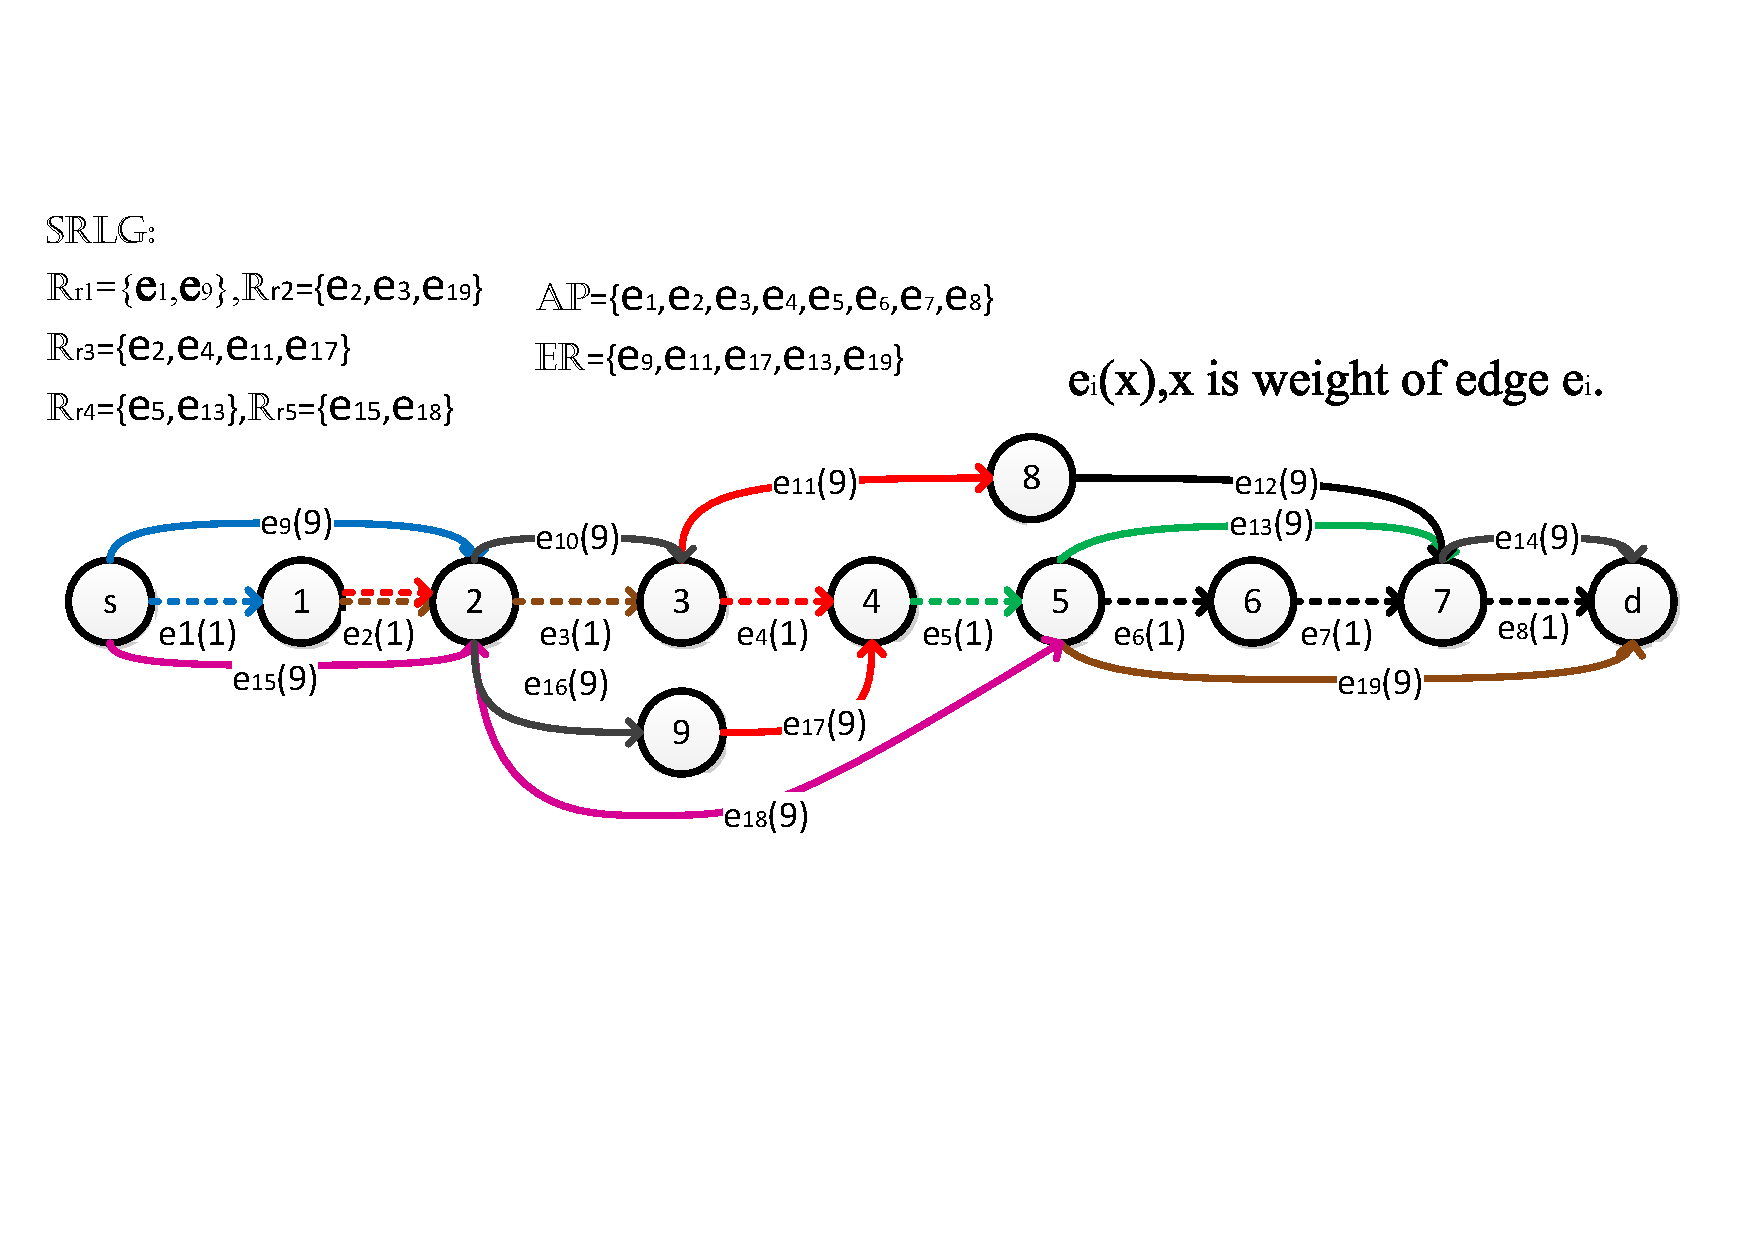
\includegraphics[width=3.5in]{franz/InitialGraph}
%\caption{$\mathbb{AP}=\{e_1,e_2,e_3,e_4,e_5,e_6,e_7,e_8\}$, $\mathbb{\mathbb{ER}}=\{e_9,e_{11},e_{17},e_{13},e_{19}\}$.  SRLGs: $\mathbb{R}_{r_1}=\{e_1,e_9\}$,$\mathbb{R}_{r_2}=\{e_2,e_3,e_{19}\}$,$\mathbb{R}_{r_3}=\{e_2,e_4,e_{11},e_{17}\}$,$\mathbb{R}_{r_4}=\{e_5,e_{13}\}$,$\mathbb{R}_{r_5}=\{e_{15},e_{18}\}$}
%\label{fig:Initial Graph}
%\end{minipage}
%\hfill
%\begin{minipage}[t]{0.3\linewidth}
%\centering
%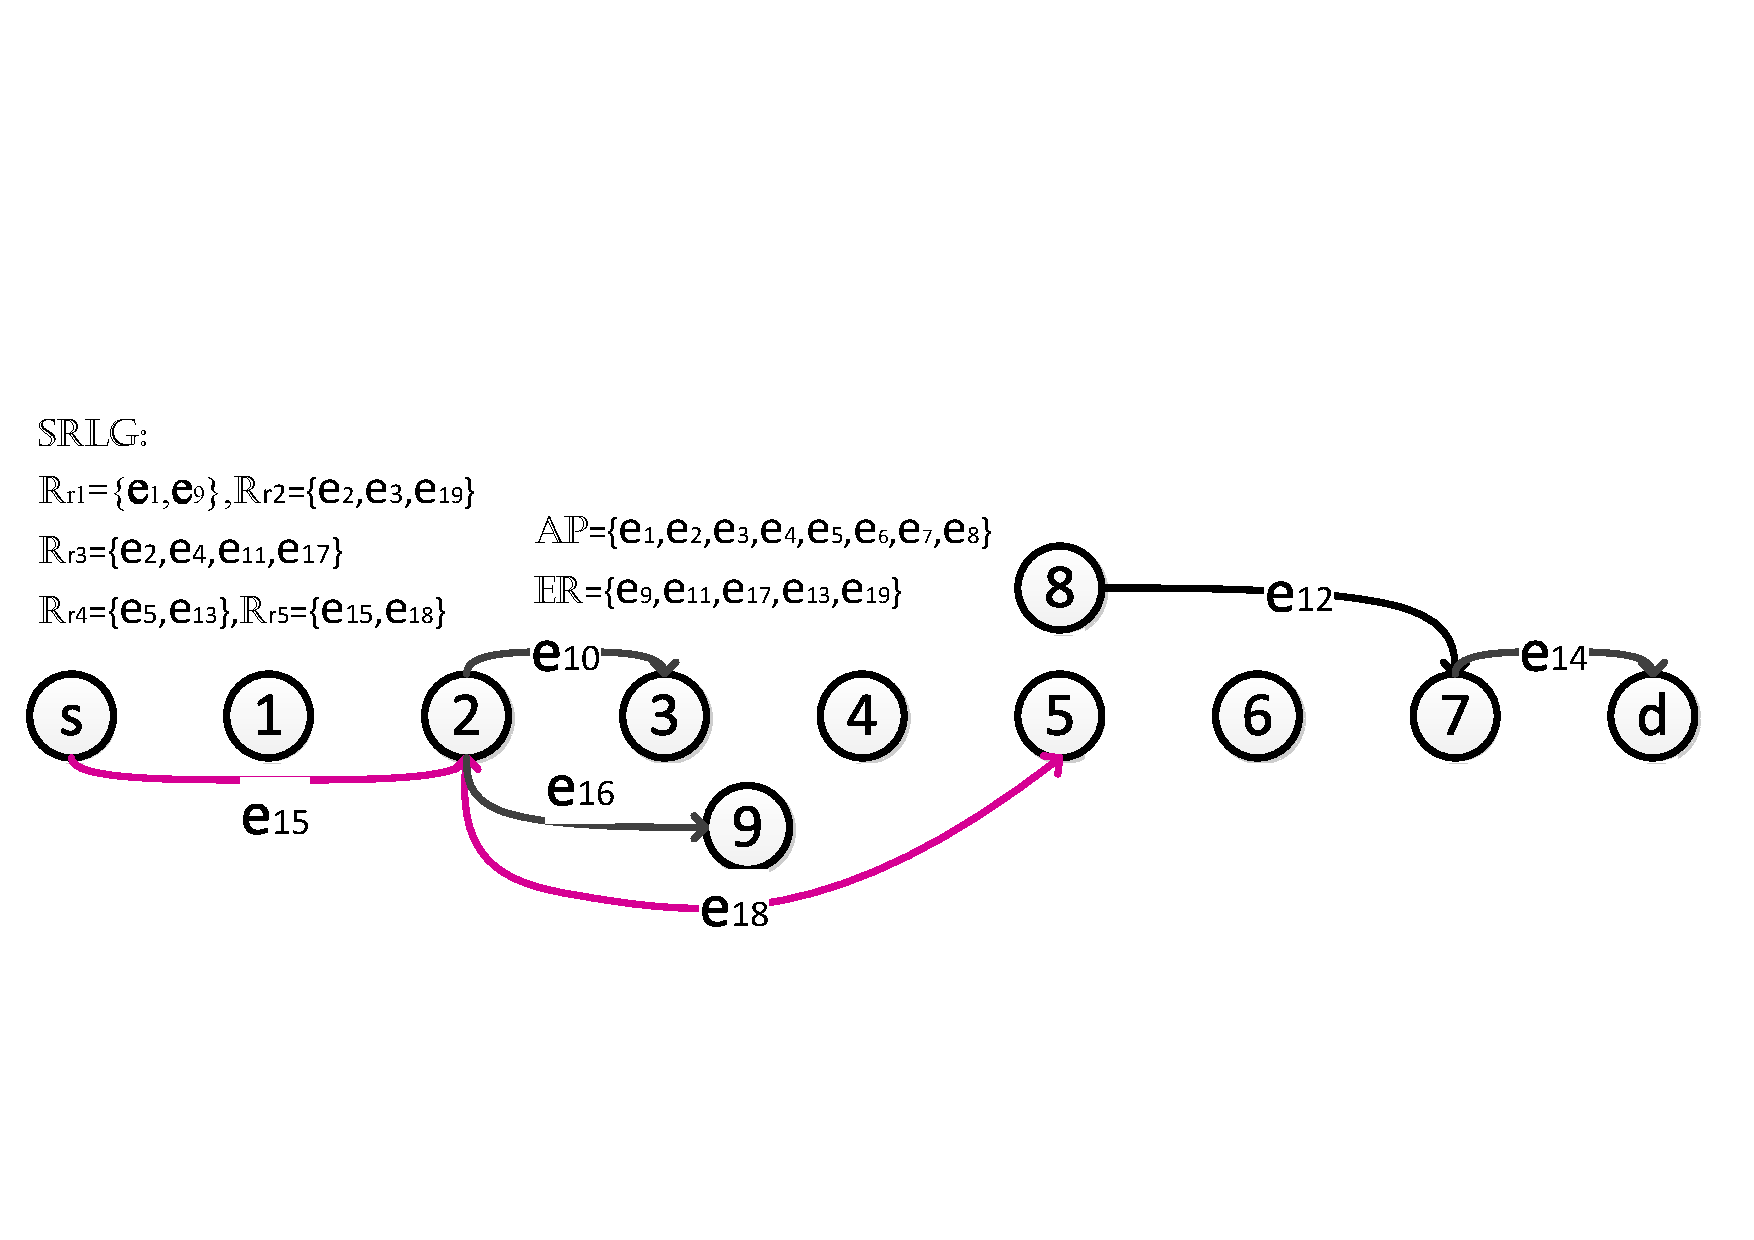
\includegraphics[width=3.5in]{franz/DeletePathGraph}
%\caption{Disconnected graph after deleting the links in $\mathbb{AP}$ and ${\mathbb{ER}}$.}
%\label{fig:DeletePathGraph}
%\end{minipage}
%\end{figure*}

%
%\begin{figure}[tp]
%  \centering
%  % Requires \usepackage{graphicx}
%  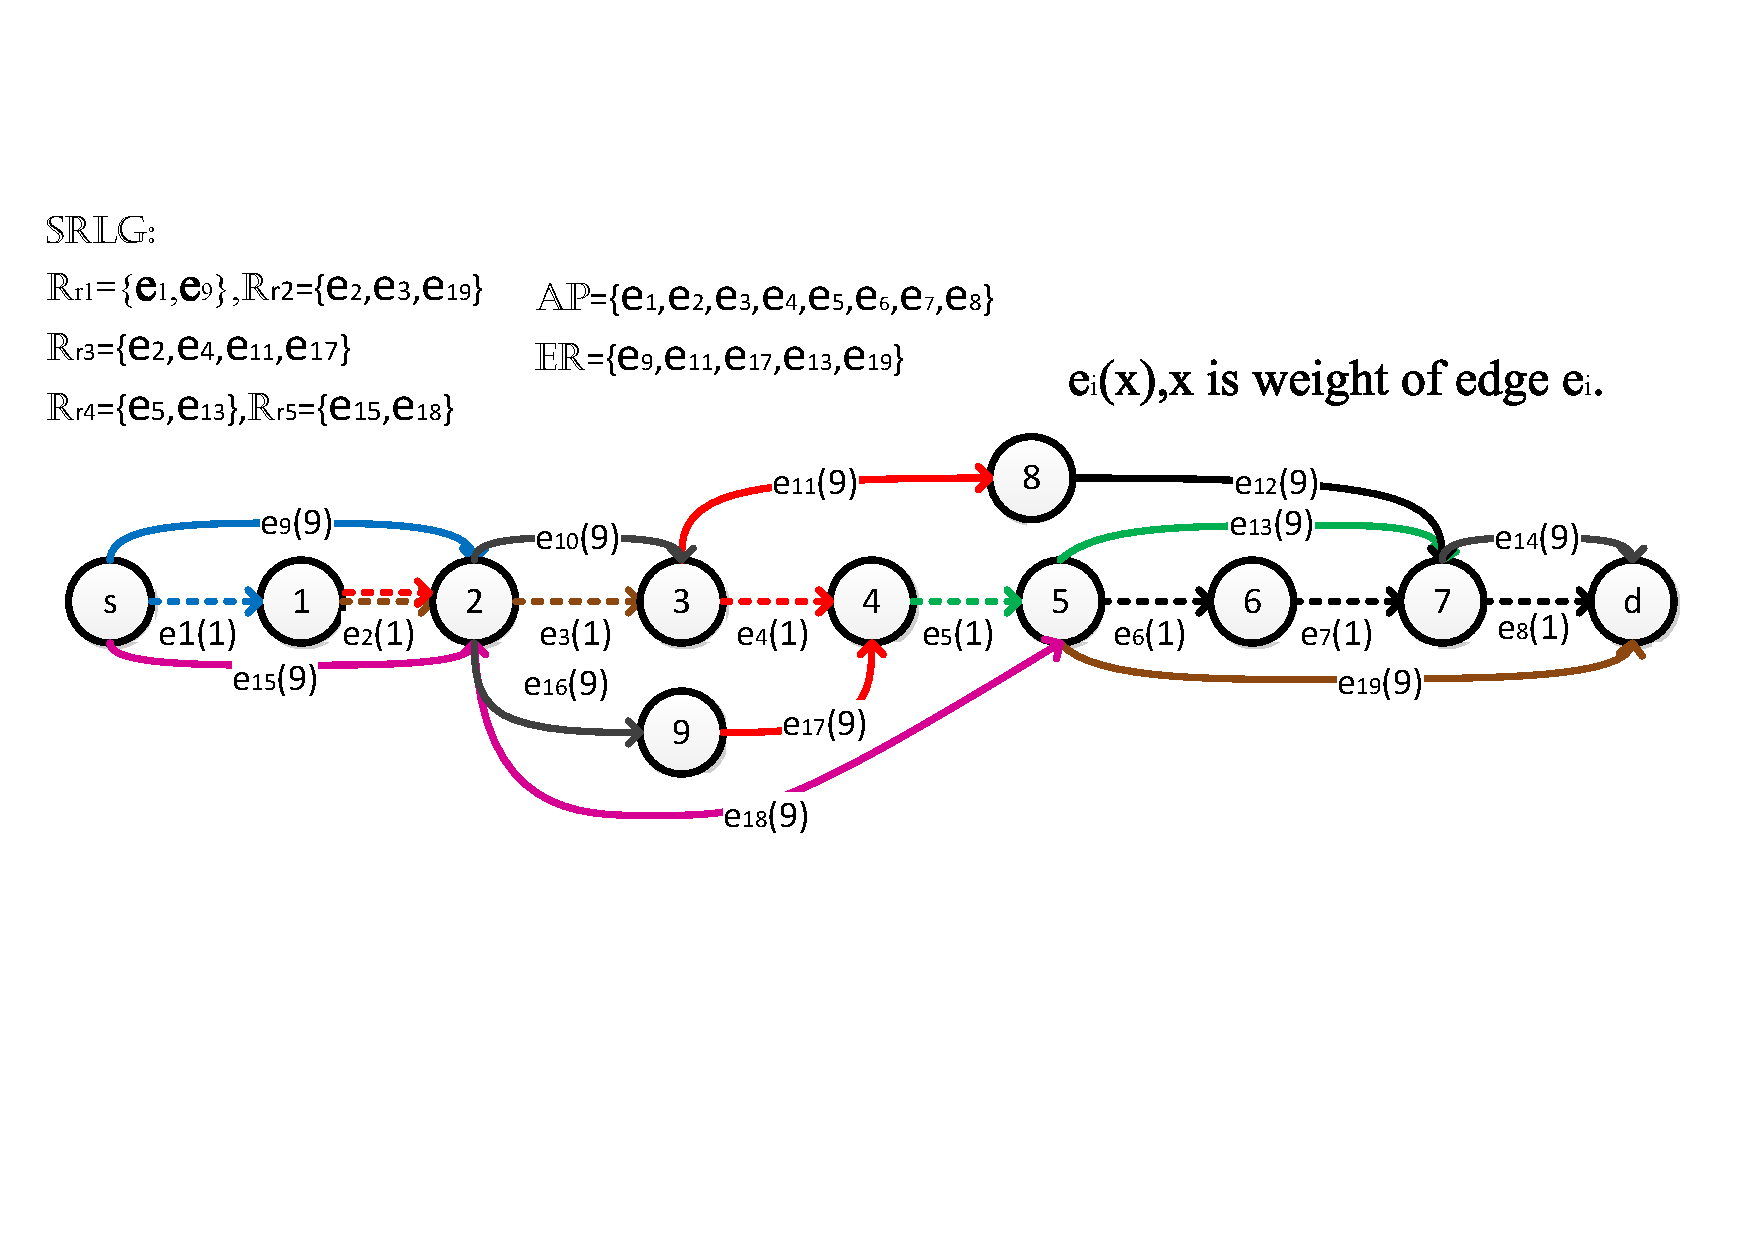
\includegraphics[width=3.6in]{franz/InitialGraph}
%  \caption{$\mathbb{AP}=\{e_1,e_2,e_3,e_4,e_5,e_6,e_7,e_8\}$, $\mathbb{\mathbb{ER}}=\{e_9,e_{11},e_{17},e_{13},e_{19}\}$. SRLGs:$\mathbb{R}_{r_1}=\{e_1,e_9\}$,$\mathbb{R}_{r_2}=\{e_2,e_3,e_{19}\}$,$\mathbb{R}_{r_3}=\{e_2,e_4,e_{11},e_{17}\}$,$\mathbb{R}_{r_4}=\{e_5,e_{13}\}$,$\mathbb{R}_{r_5}=\{e_{15},e_{18}\}$}\label{fig:Initial Graph}
%\end{figure}
%\begin{figure}[tp]
%  \centering
%  % Requires \usepackage{graphicx}
%  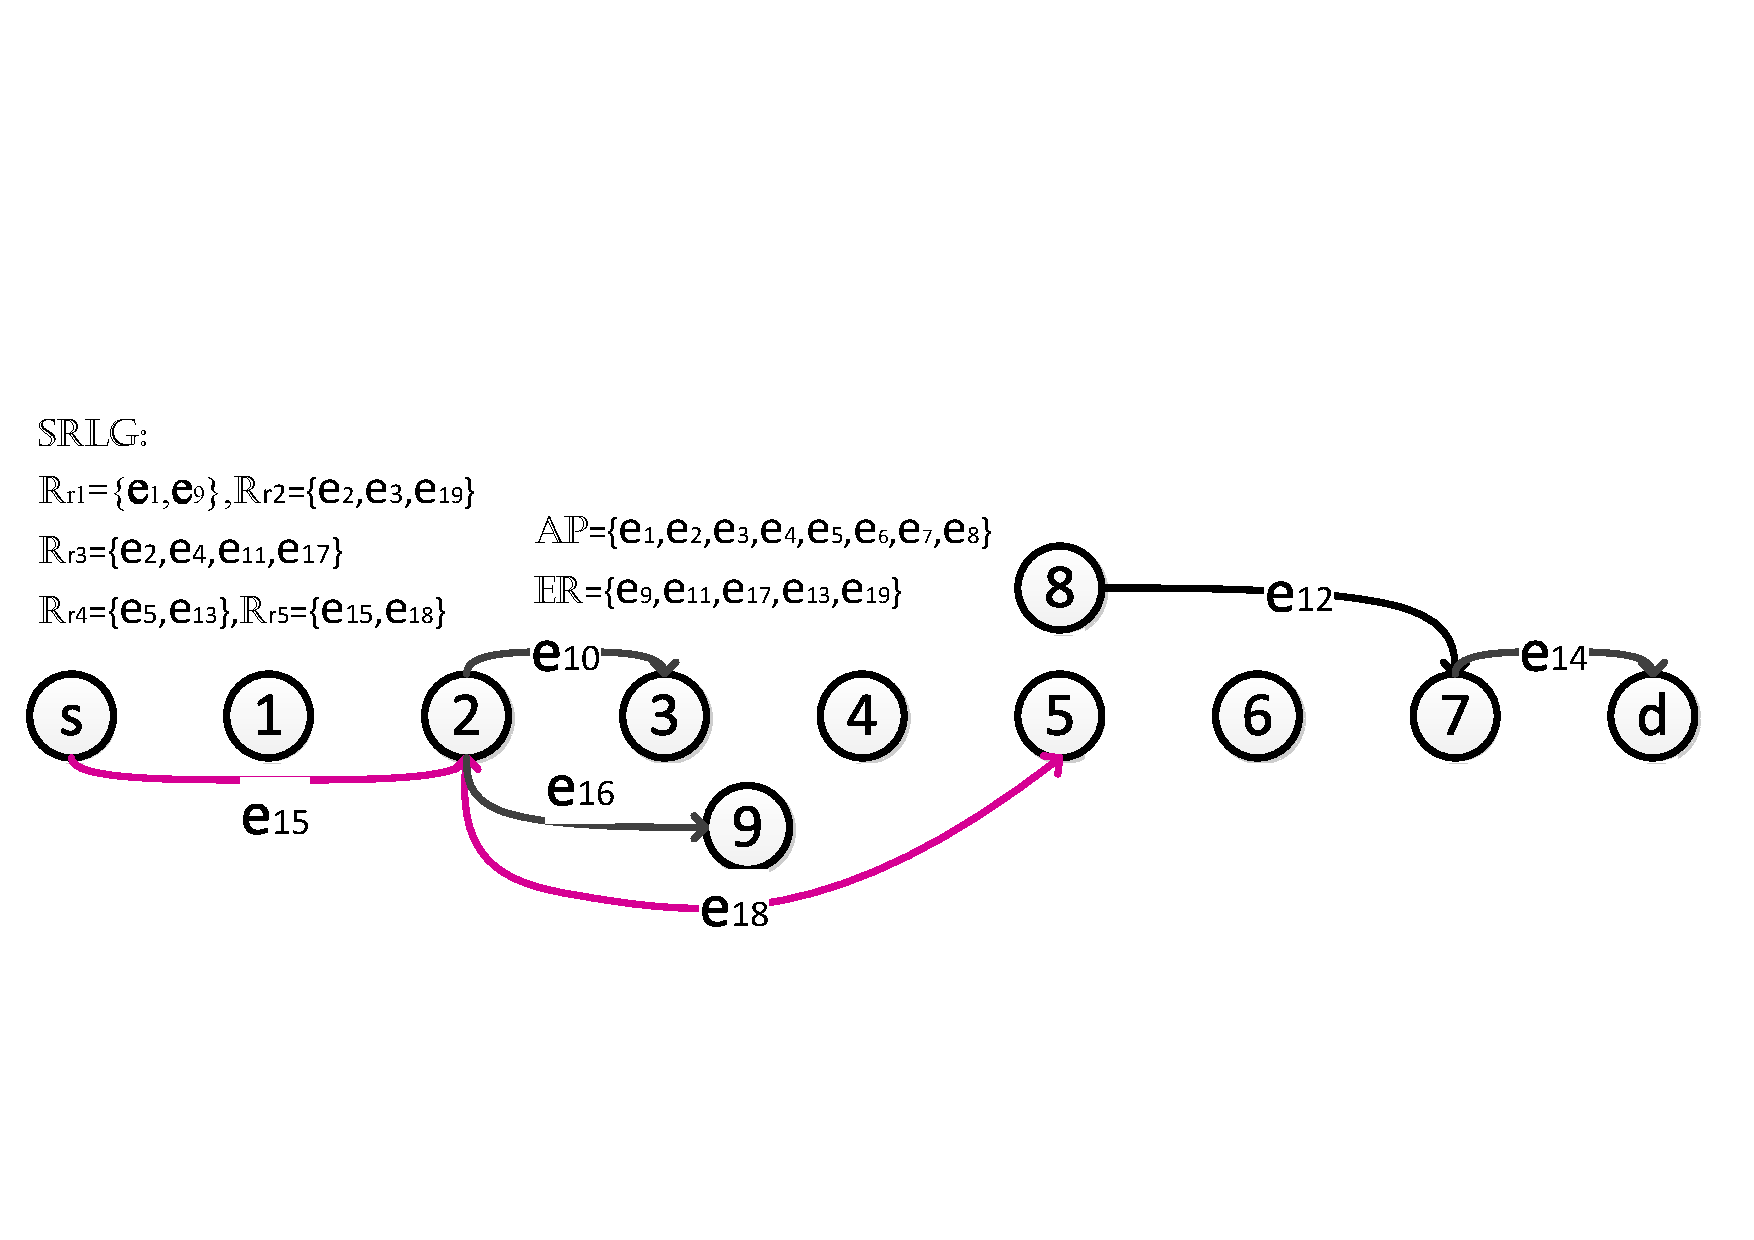
\includegraphics[width=3.4in]{franz/DeletePathGraph}
%  \caption{Disconnected graph after deleting the links in $\mathbb{AP}$ and ${\mathbb{ER}}$.}
%  \label{fig:DeletePathGraph}
%\end{figure}

\begin{figure*}[tp]
  \centering
  % Requires \usepackage{graphicx}
  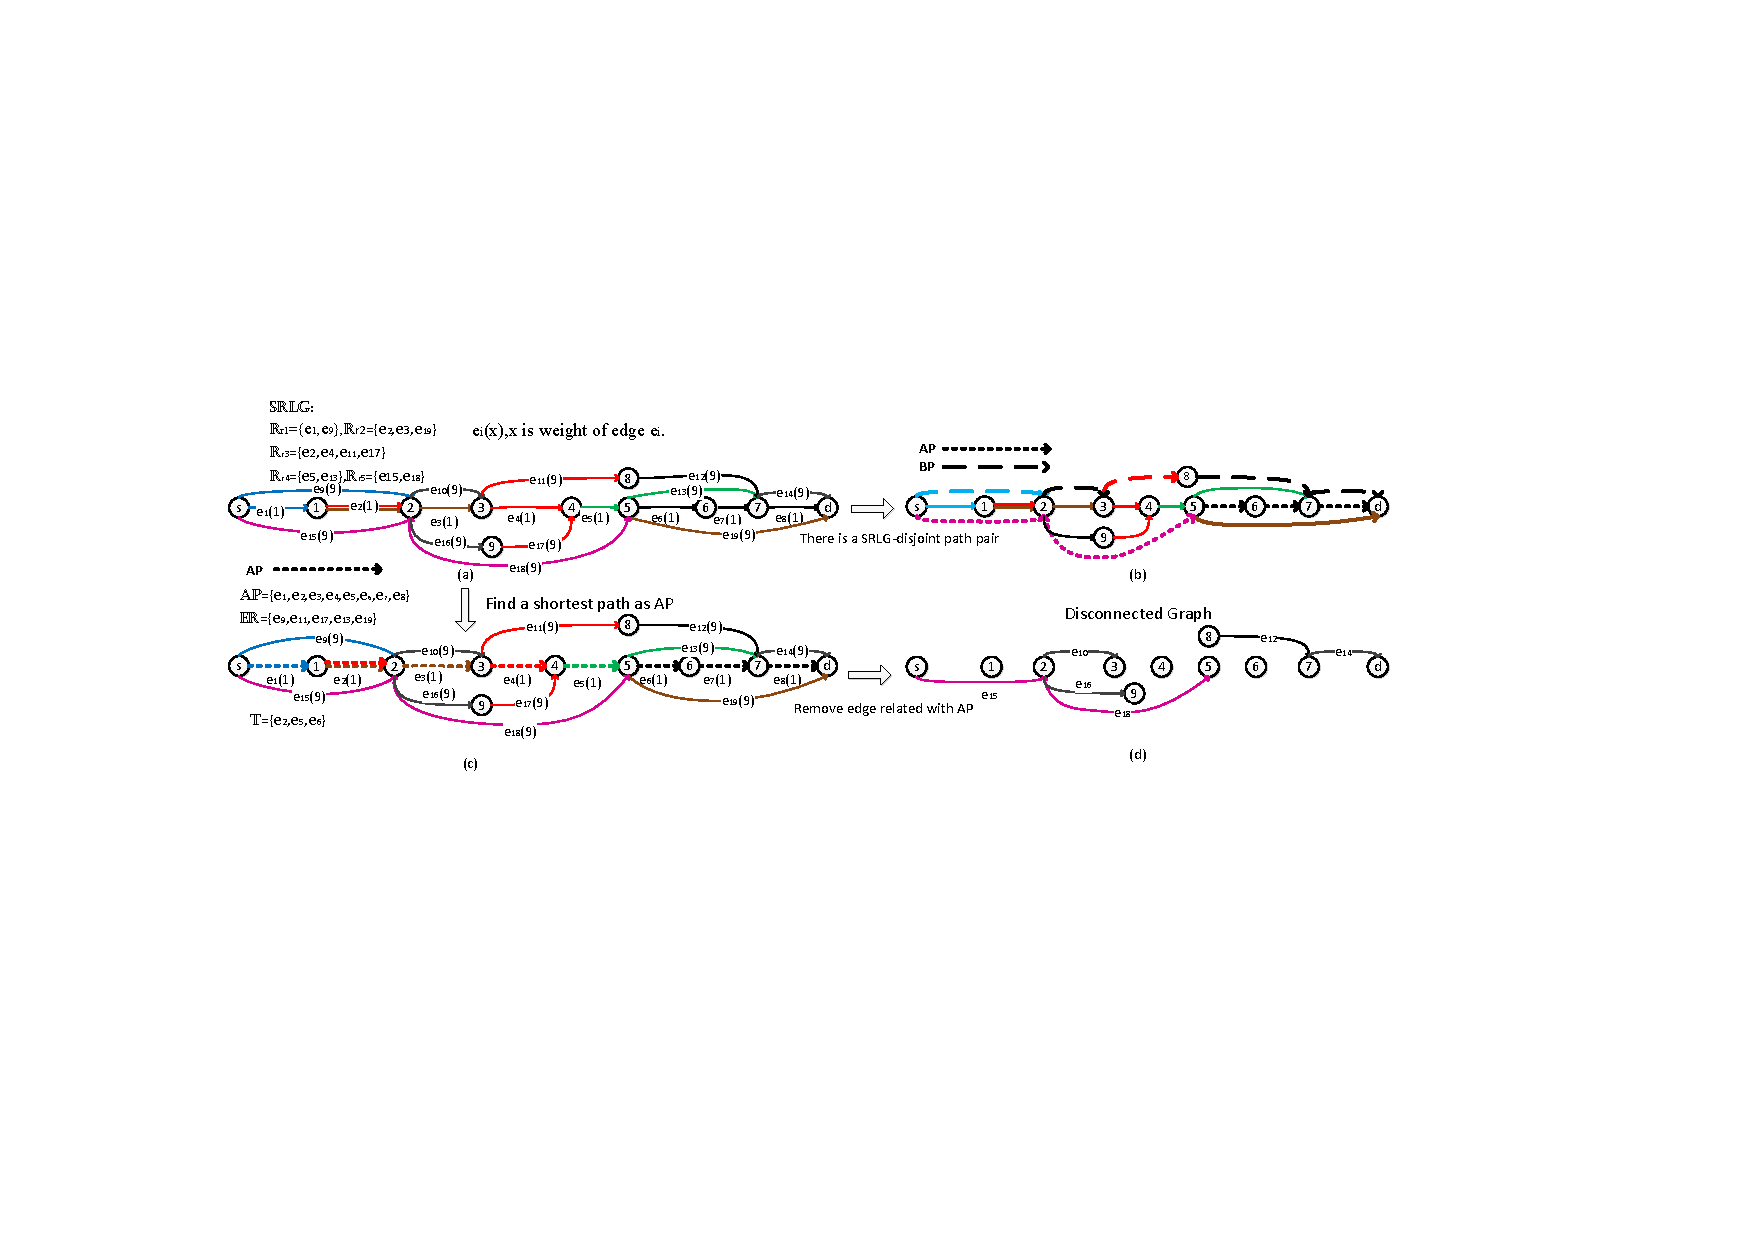
\includegraphics[width=7.2in]{franz/CompositeGraph}
  \caption{(a) A graph with five SRLGs: $\mathbb{R}_{r_1}=\{e_1,e_9\}$,$\mathbb{R}_{r_2}=\{e_2,e_3,e_{19}\}$,$\mathbb{R}_{r_3}=\{e_2,e_4,e_{11},e_{17}\}$,$\mathbb{R}_{r_4}=\{e_5,e_{13}\}$,$\mathbb{R}_{r_5}=\{e_{15},e_{18}\}$. (b)AP and BP in the graph. (c) The shortest weight path AP in the graph. $\mathbb{AP}=\{e_1,e_2,e_3,e_4,e_5,e_6,e_7,e_8\}$, $\mathbb{\mathbb{ER}}=\{e_9,e_{11},e_{17},e_{13},e_{19}\}$. (d)  Graph after deleting the links in $\mathbb{AP}$ and ${\mathbb{ER}}$. }
  \label{fig:CompositeGraph}
\end{figure*}


%\subsection{Problem analysis}
%\label{sec:NPC proof}
%\begin{theorem}
%\label{le:lemma1}
%    The Min-Min SRLG-disjoint path problem is NP-complete.
%\end{theorem}
%
%Proof: Due to the limited space, the proof is omitted.

\subsection{Problem analysis}
\label{sec:NPC proof}
\begin{theorem}
\label{le:lemma1}
    The Min-Min SRLG-disjoint path problem is NP-complete.
\end{theorem}

\begin{proof}
According to \cite{bhatia2006finding}, the Min-Min link-disjoint path problem is NP-complete.  It is a sub-problem of Min-Min SRLG-disjoint path problem. Denote our Min-Min SRLG-disjoint path problem as $A$. The complexity of  problem $A$ is denoted as $C(A)$, we have $NP-complete\leq C(A) $.

To prove that $C(A)$ also satisfies that $C(A) \leq NP-complete$ and thus $C(A)= NP-complete$, we build another problem $B$:  finding two SRLG-disjoint paths with the minimum path weight less than or equal to $M$. Obviously, we have $0< M \le \sum\limits_{e_i\in \mathbb{E}}w_{e_i}$ as the path weight is  the sum of the link weights along the path. \note{What is the last item? The weight of all links in the network? Then your explanation needs to be more clear. Do you want to say the summation of weights from links on a path is smaller than the summation of weights from links of the whole network?}

\revtao{Using a} classical binary search method, we can find that the solution of  problem $A$ can be found by testing the solution of problem $B$ with different $M$ \rev{vales}.  Fig.\ref {fig:binarySearch} uses an example to illustrate the binary search method. \del{In this example,} The link weight \note{So confusing. You said M is the path weight. Why it is the link weight now?} is denoted by an integer, $0 < M \le 10$, and the minimum path weight under  problem $A$ is $m=6$. To find the optimal solution of problem $A$ with $m=6$ using problem $B$, we \del{firstly} \rev{first} test whether there exists solution for problem $B$ with $M=5$. As $m=6$ and we can not find the solution for problem $B$ with $M=5$, \del{therefore,} \note{Why do you always add therefore after you use as? They have the same meaning is a repetition. Such a low level elementary school grammar error.} the solution should \rev{fall into} $5< M \le 10$. \del{Thus,} We  further test whether there exists \rev{a} solution for problem $B$ with $M=7$, and then $M=6$. After we test problem $B$ with $M=6$, the optimal solution of  problem $A$ can be found. \rev{Depending on the time complexity of the simple classical binary search,} \del{of polynomial,} the solution of problem $A$ can be searched based on the solution of problem $B$. Therefore, we have that \rev{the complexity level of problem $B$}  is equal to that of problem $A$.

\revtao{Problem} $B$ can be reducible to the NP-hard halting problem. Moreover, given any two paths, it is easy (in polynomial time) to identify whether they are SRLG-disjoint and satisfy that the minimum path weight is less than or equal to $M$.
As \rev{$A$'s complexity level is equal to that of $B$}, we have $C(A)=C(B) \le NP-complete$. Therefore, $C(A)=NP-complete$.
\note{Is NP-hard complexity higher or NP-Complete?}





\end{proof}
\begin{figure}[tp]
  \centering
  % Requires \usepackage{graphicx}
  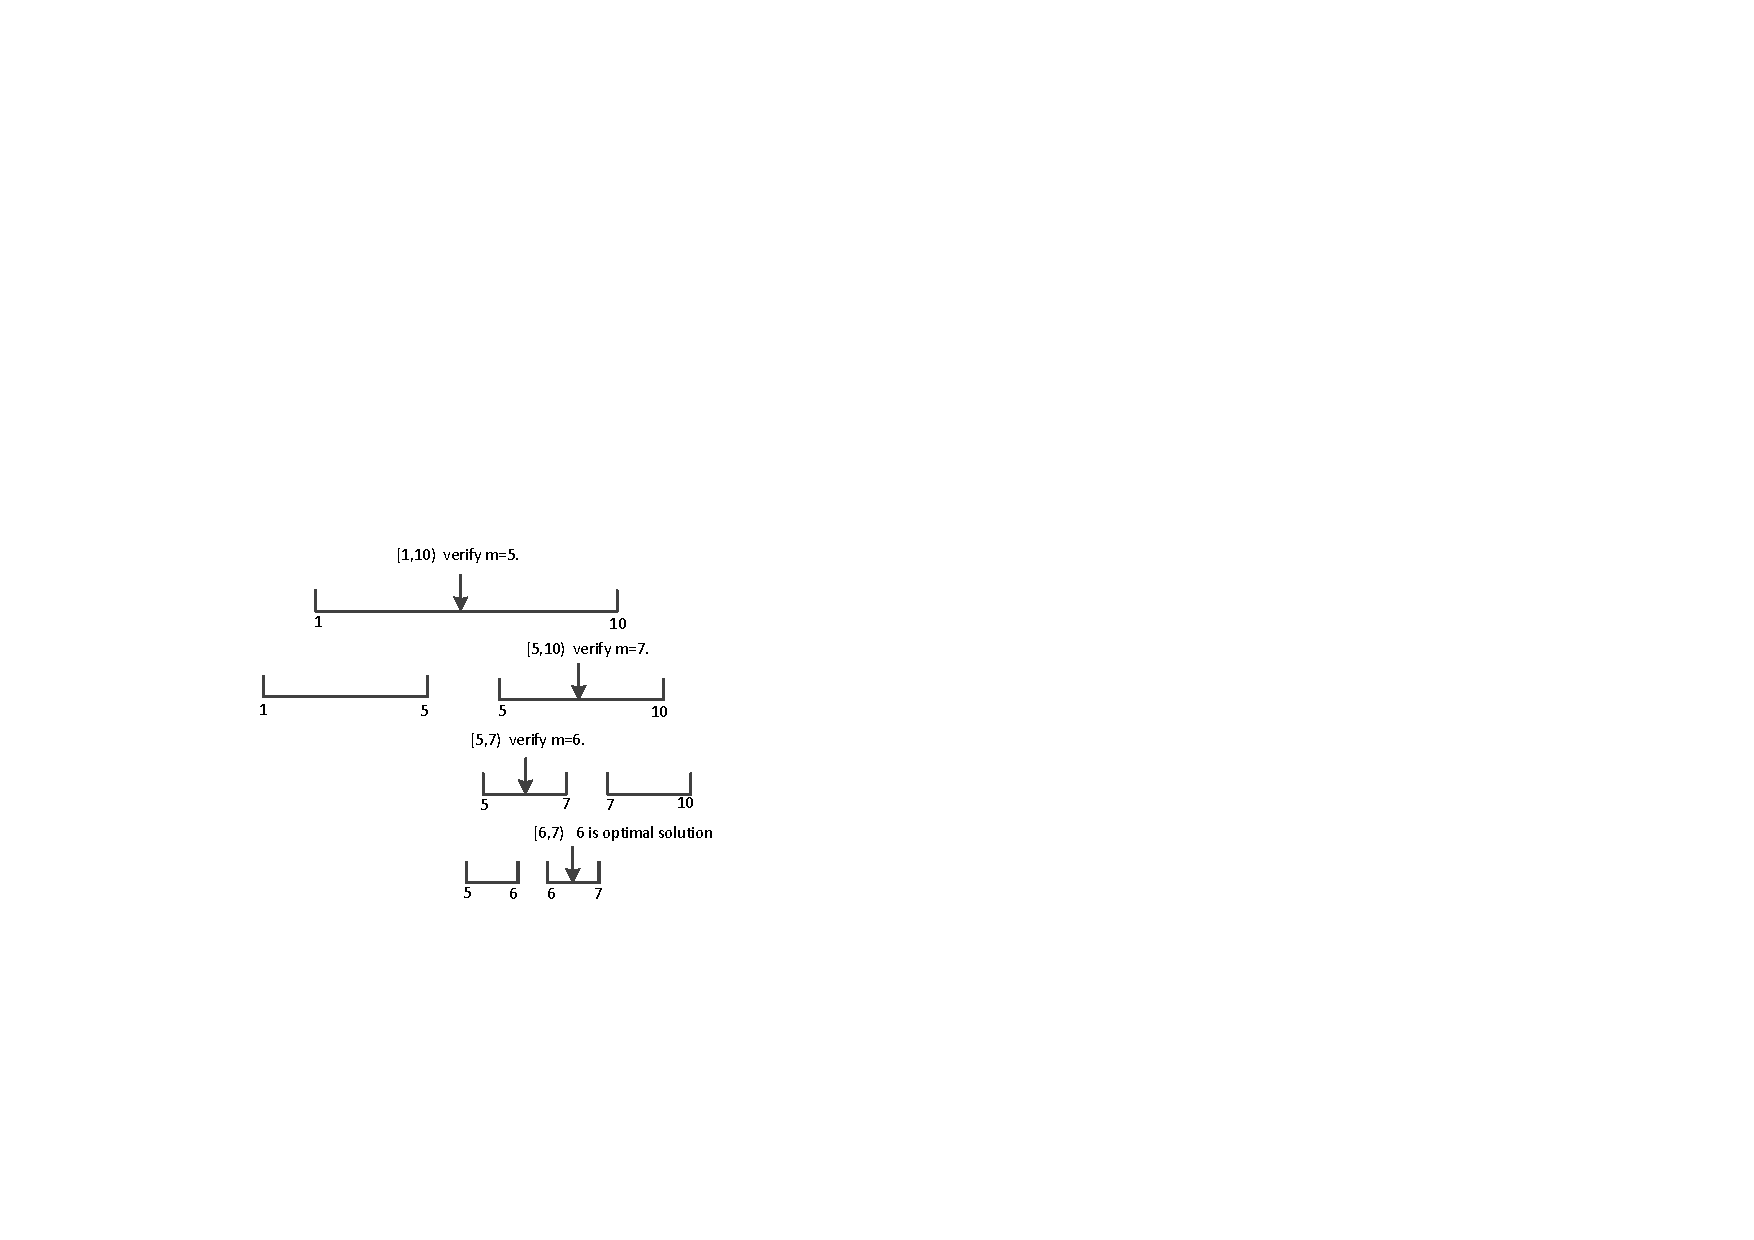
\includegraphics[width=3.0in]{franz/binarySearch}
  \caption{Request optimal solution of Problem A  through Binary search method }
  \label{fig:binarySearch}
\end{figure}
